\documentclass[12pt,compress]{beamer}
\usepackage{ifthen,verbatim}

\title{Tracks Seeded by Electron SuperClusters}
\author{Jim Pivarski}
\institute{Cornell University}
\date{28 July, 2006}

\setbeamertemplate{navigation symbols}{}
\setbeamertemplate{headline}{\includegraphics[height=1 cm]{cmslogo} \hfill
\begin{minipage}{8 cm}
\vspace{-0.75 cm} \small
\begin{center}
\ifthenelse{\equal{\insertpagenumber}{0}}{}{\insertsection\ (\insertpagenumber/\pageref{numpages})}
\end{center}
\end{minipage} \hfill \includegraphics[height=1 cm]{lepplogo}}

\xdefinecolor{verylightgray}{rgb}{0.95,0.95,0.95}
\beamertemplateshadingbackground{verylightgray}{white}

\begin{document}
\addtocounter{page}{-1}
\frame{\titlepage}
\section*{Tracks from Electrons --- Jim Pivarski}

\begin{frame}
\frametitle{Hits passed to TrackProducer}

\begin{center}
\includegraphics[width=0.7\linewidth]{event_display_banded}
\end{center}

\small
\begin{itemize}
\item Linear band in $\phi(r)$ ($\Delta \phi$ $=$ 10 mrad) from SuperCluster (\textcolor{red}{red})
\item All rphi (black) and stereo (\textcolor{blue}{blue}) SiStrip hits within band are copied to TrackCandidate
\item Also has a trajectory state, valid at position of innermost hit
\end{itemize}
\end{frame}

\begin{frame}[fragile]
\frametitle{C++ snippet}
\tiny
\begin{verbatim}
edm::OwnVector<TrackingRecHit> outputHits;

...
outputHits.push_back(((TrackingRecHit*)(*hit))->clone());
...

// Initial uncertainty for tracking
AlgebraicSymMatrix errors(5,1);  // makes identity 5x5 matrix, indexed from (1,1) to (5,5)
errors(1,1) = 3.;                // uncertainty**2 in 1/momentum
errors(2,2) = 0.01;              // uncertainty**2 in lambda (lambda == pi/2 - polar angle theta)
errors(3,3) = 0.0001;            // uncertainty**2 in phi
errors(4,4) = 0.01;              // uncertainty**2 in x_transverse (where x is in cm)
errors(5,5) = 0.01;              // uncertainty**2 in y_transverse (where y is in cm)

outputHits.sort(TrackingRecHitLessFromGlobalPosition(((TrackingGeometry*)(tracker)), alongMomentum));

TrajectoryStateOnSurface state(
         GlobalTrajectoryParameters(position, momentum, -1, magneticField),
         CurvilinearTrajectoryError(errors),
         tracker->idToDet(innerhit->geographicalId())->surface());

TrajectoryStateTransform transformer;
PTrajectoryStateOnDet* PTraj = transformer.persistentState(state, innerhit->geographicalId().rawId());
TrajectorySeed trajectorySeed(*PTraj, outputHits, alongMomentum);
trackCandidateOut.push_back(TrackCandidate(outputHits, trajectorySeed, *PTraj));
\end{verbatim}
\end{frame}

\begin{frame}[fragile]
\frametitle{.cfg snippet}
\tiny
\begin{verbatim}
# KFUpdatoerESProducer
include "TrackingTools/KalmanUpdators/data/KFUpdatorESProducer.cfi"

# Chi2MeasurementEstimatorESProducer
include "TrackingTools/KalmanUpdators/data/Chi2MeasurementEstimatorESProducer.cfi"

# KFTrajectoryFitterESProducer
include "TrackingTools/TrackFitters/data/KFTrajectoryFitterESProducer.cfi"

# KFTrajectorySmootherESProducer
include "TrackingTools/TrackFitters/data/KFTrajectorySmootherESProducer.cfi"

# KFFittingSmootherESProducer
include "TrackingTools/TrackFitters/data/KFFittingSmootherESProducer.cfi"

# PropagatorWithMaterialESProducer
include "TrackingTools/MaterialEffects/data/MaterialPropagator.cfi"

# PropagatorWithMaterialESProducer
include "TrackingTools/MaterialEffects/data/OppositeMaterialPropagator.cfi"

# TransientTrackingBuilder
include "RecoTracker/TransientTrackingRecHit/data/TransientTrackingRecHitBuilder.cfi"

# TrackProducer
include "RecoTracker/TrackProducer/data/CTFFinalFitWithMaterial.cfi"
replace CTFWMaterial.src = "findElectronsInSiStrips"
\end{verbatim}
\end{frame}

\begin{frame}
\frametitle{75\% efficiency!}
\small
\begin{itemize}
\item 284 fitted tracks from 378 track candidates
\item 50 GeV electron-gun with $\eta = 0$
\end{itemize}
\begin{center}
\includegraphics[width=0.7\linewidth]{numhits_withtrack_overlay}

overlay successful events on all candidate events (\# hits)
\end{center}
\end{frame}

\begin{frame}
\frametitle{$\phi$ resolution is 12 mrad}
\begin{center}
\includegraphics[width=0.8\linewidth]{dphi_track}
\end{center}
\end{frame}

\begin{frame}
\frametitle{$\eta$ resolution is 0.03}
\begin{center}
\includegraphics[width=0.8\linewidth]{deta_track}
\end{center}
\end{frame}

\begin{frame}
\frametitle{$z$ resolution is 40 mm}
\begin{center}
\includegraphics[width=0.8\linewidth]{dz_track}
\end{center}
\end{frame}

\begin{frame}
\frametitle{$p_T$ has a low-energy tail}
\begin{center}
\includegraphics[width=0.8\linewidth]{pt_track}
\end{center}
\end{frame}

\begin{frame}
\frametitle{$p_T|_{\mbox{\scriptsize outer}}$ has a bigger low-energy tail (good)}
\begin{center}
\includegraphics[width=0.8\linewidth]{pt_trackouter}
\end{center}
\end{frame}

\begin{frame}
\frametitle{$p_T|_{\mbox{\scriptsize inner}} - p_T|_{\mbox{\scriptsize outer}}$ is symmetric (huh?)}
\begin{center}
\includegraphics[width=0.8\linewidth]{inoutpt}
\end{center}
\end{frame}

\begin{frame}
\frametitle{$\phi|_{\mbox{\scriptsize inner}} - \phi|_{\mbox{\scriptsize outer}}$ is too big by a factor of two}
\begin{center}
\includegraphics[width=0.8\linewidth]{inoutphi}
\end{center}
\end{frame}

\begin{frame}
\frametitle{Why do I say that?}
\begin{center}
\includegraphics[width=0.8\linewidth]{dphi_supercluster}
\end{center}
\end{frame}

\begin{frame}[fragile]
\begin{minipage}{\linewidth}
\frametitle{I also have a factor of two error in $\phi|_{\mbox{\scriptsize inner}} - \phi|_{\mbox{\scriptsize outer}}$}
\tiny
\begin{verbatim}
// This comes from Jackson p. 581-2, a little geometry, and a FUDGE
// FACTOR of two in the denominator.  Why is that factor of two correct?
// (It's not confusion about radius vs. diameter in the definition of
// curvature.)

double phiVsRSlope = -3.00e-3 * chargeHypothesis * magneticField->inTesla().z() / pT / 2.;
\end{verbatim}
\end{minipage}

\vfill
The $\phi|_{\mbox{\scriptsize inner}} - \phi|_{\mbox{\scriptsize
outer}}$ I calculate is 2$\times$ larger than the simulated track.
Could it be that

\vspace{0.25 cm}
\newcounter{Lcount}
\begin{list}{\alph{Lcount}) }
{\usecounter{Lcount}}
\item electron-gun $p_T$ is half of the value requested, and
\item reco::Track reports $p_T$ as twice the value fitted?
\end{list}
\end{frame}

\begin{frame}
\frametitle{$\eta|_{\mbox{\scriptsize inner}} - \eta|_{\mbox{\scriptsize outer}}$ has an asymmetric satellite}
\begin{center}
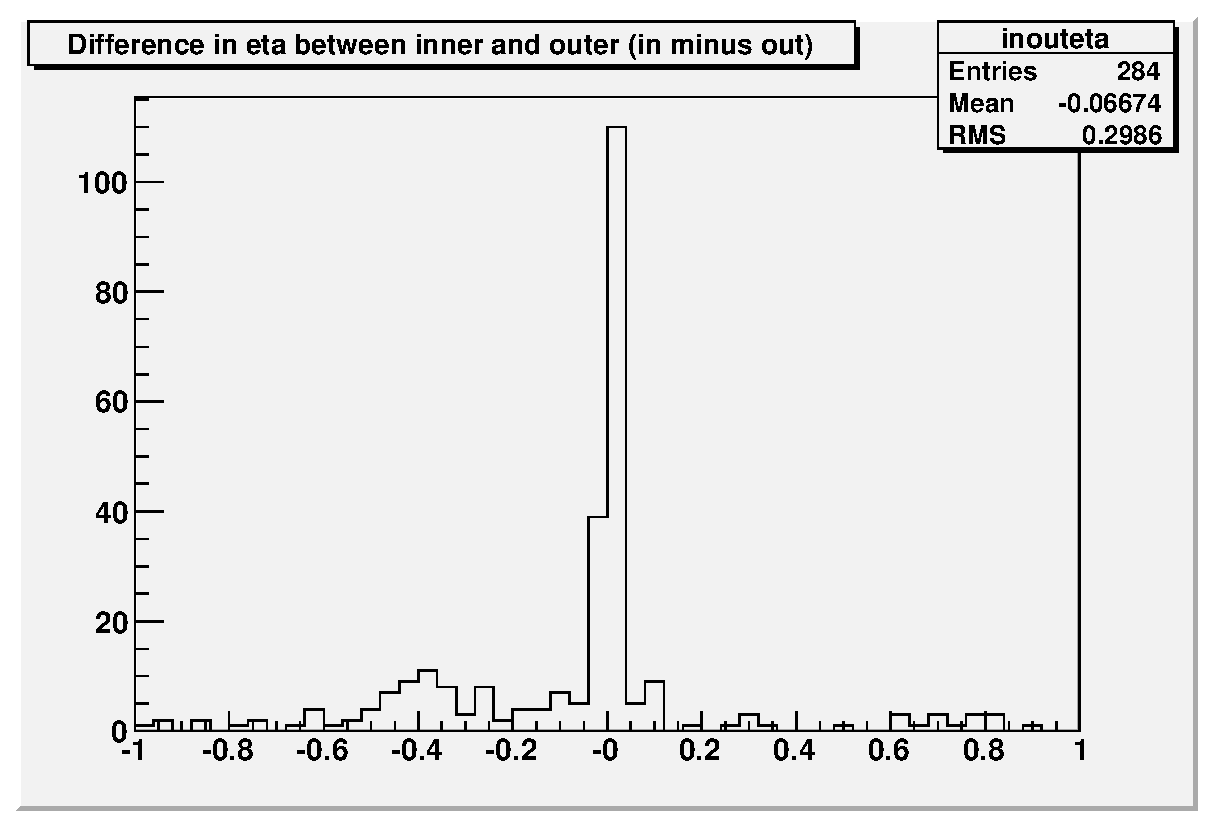
\includegraphics[width=0.8\linewidth]{inouteta}
\end{center}
\end{frame}

\begin{frame}
\frametitle{$\chi^2/N_{\mbox{\scriptsize dof}}$ is still too large (I'm passing too many hits)}
\begin{center}
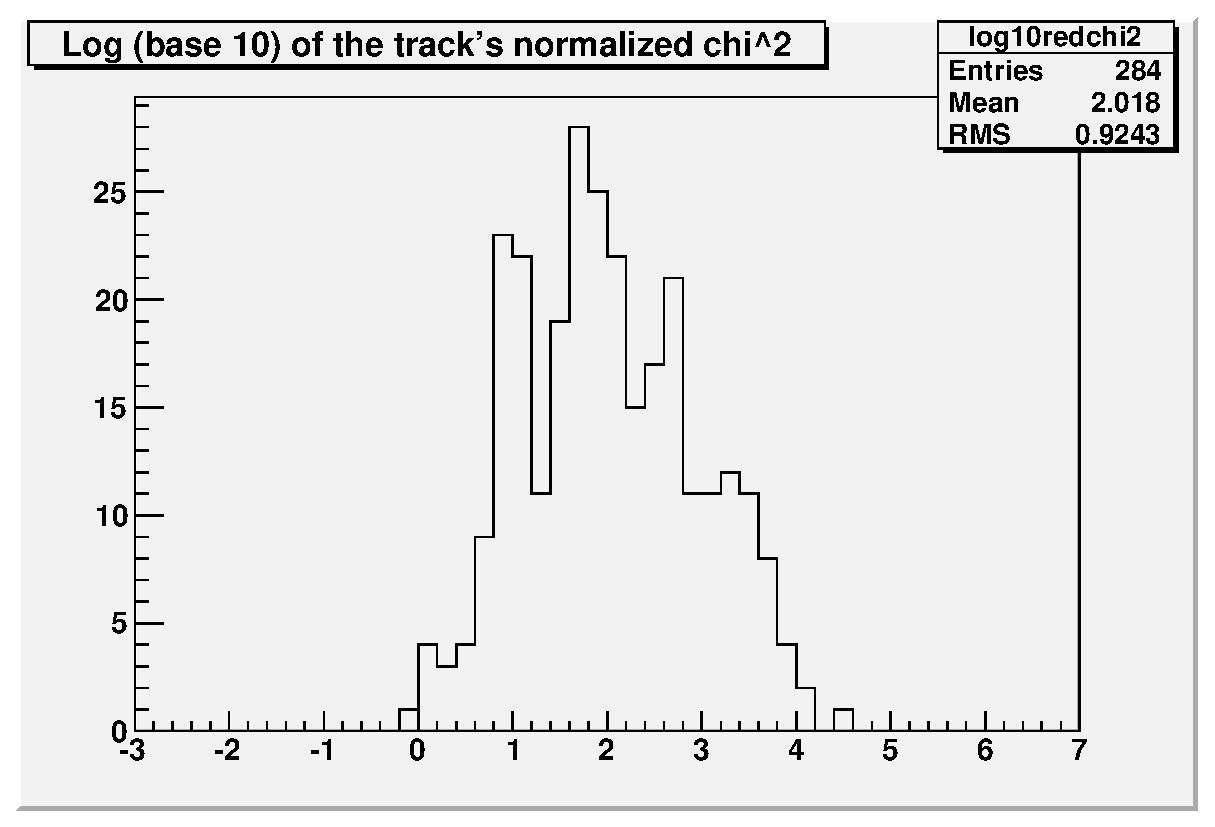
\includegraphics[width=0.8\linewidth]{log10redchi2}
\end{center}
\end{frame}

\begin{frame}
\frametitle{Why is \#hits $-$ $N_{\mbox{\scriptsize dof}}$ not constant (why not 5)?}
\begin{center}
\includegraphics[width=0.8\linewidth]{numparameters}
\end{center}
\end{frame}

\begin{frame}
\frametitle{First Impressions}
\label{numpages}

\begin{itemize}\setlength{\itemsep}{0.5 cm}
\item 75\% efficiency and $\chi^2$ may be due to extraneous hits
\item Strange features in inner $-$ outer track parameters
\item I also have a factor of two error converting between $p_T$ and $\phi|_{\mbox{\scriptsize inner}} - \phi|_{\mbox{\scriptsize outer}}$
\item {\small \tt track.found()} {\small \tt ==} \#input hits {\small \tt !=} {\small \tt track.ndof()+5}
\end{itemize}

\end{frame}

\end{document}
